% Models and search heuristics of the approximate high level synthesis in axc-simulator, explained step by step with
% the Sobel kernel as the running example. Single file; compile with pdflatex (two passes for the references).
\documentclass[11pt,a4paper]{article}
\usepackage[T1]{fontenc}
\usepackage[utf8]{inputenc}
\usepackage{lmodern}
\usepackage[margin=2.3cm]{geometry}
\usepackage{amsmath,amssymb}
\usepackage{algorithm}
\usepackage{algpseudocode}
\usepackage[table]{xcolor}
\usepackage{array}
\usepackage{listings}
\usepackage{tikz}
\usetikzlibrary{positioning,arrows.meta}
\usepackage[hidelinks]{hyperref}
\definecolor{tabAzul}{RGB}{31,78,121}

\algrenewcommand\algorithmicrequire{\textbf{Input:}}
\algrenewcommand\algorithmicensure{\textbf{Output:}}
\newcommand{\E}{\mathbb{E}}
\newcommand{\Var}{\operatorname{Var}}
\newcommand{\Cost}{C}
\newcommand{\Feas}{\mathcal{F}}

\lstset{language=C, basicstyle=\ttfamily\small, numbers=left, numberstyle=\tiny\color{gray}, columns=fullflexible,
  keywordstyle=\color{tabAzul}\bfseries, commentstyle=\color{gray}, frame=single, rulecolor=\color{gray!50},
  morekeywords={u8,i16}, xleftmargin=1.5em}

% Example: a shaded block that applies the definition just given to the running example.
\newcommand{\examplebox}[2]{\par\medskip\noindent\colorbox{tabAzul!6}{\begin{minipage}{\dimexpr\linewidth-2\fboxsep}
  \textbf{Example (#1).}\ #2\end{minipage}}\par\medskip}

\title{Approximate high level synthesis in axc-simulator:\\ cost model, error model and search heuristics,\\ step by step}
\author{Prof. Dr. Tiago Almeida}
\date{}

\begin{document}
\maketitle

\section{Overview}

The simulator answers one question: which approximate arithmetic unit should each addition, subtraction and
multiplication of a C kernel use, so that the hardware is as cheap as possible while the output error stays within a
limit? It never runs a logic synthesis tool inside the search. Instead, it chains six steps, each explained in one
section of this text:

\begin{enumerate}
  \item \textbf{Elaboration} (Section~\ref{sec:elab}): the kernel becomes data flow graphs, and each approximable
    operation gets a width and a list of library units.
  \item \textbf{Profile} (Section~\ref{sec:elab}): the kernel runs once, exactly, on the input data; the operands of
    every operation are sampled.
  \item \textbf{Cost} (Section~\ref{sec:cost}): a model of scheduling, binding and the library gives area, LUTs,
    energy and latency of any assignment of units.
  \item \textbf{Error estimate} (Section~\ref{sec:err}): a static model gives the mean and the mean square of the error
    at every output, without running the approximate kernel.
  \item \textbf{Search} (Section~\ref{sec:search}): a heuristic looks for the cheapest assignment whose estimated
    error satisfies the constraint.
  \item \textbf{Verification} (Section~\ref{sec:verify}): the best points are executed bit by bit with the
    approximate units, and the first one whose measured error satisfies the constraint is the answer.
\end{enumerate}
Section~\ref{sec:results} compares the heuristics on the running example.

Every definition below is followed by an example on the same kernel, the Sobel edge detector of the simulator
(Listing~\ref{lst:sobel}). The numbers in the examples are the ones the simulator prints for this kernel with a
5~ns clock, the sky130 library, the area objective and the default test image of $192 \times 192$ pixels.

\begin{lstlisting}[caption={Sobel kernel (the line numbers are the ones the simulator reports).},label={lst:sobel},float=t]
// Sobel edges: |Gx| + |Gy| (L1 norm), divided by 4 and saturated at 255.
#define W 192
#define H 192

void sobel(u8 in[H][W], u8 out[H][W]) {
#pragma HLS array_partition variable=in type=cyclic factor=3 dim=1
rows:
    for (int y = 1; y < H - 1; y++) {
cols:
        for (int x = 1; x < W - 1; x++) {
#pragma HLS pipeline II=1
            i16 gx = in[y - 1][x + 1] + 2 * in[y][x + 1] + in[y + 1][x + 1]
                   - in[y - 1][x - 1] - 2 * in[y][x - 1] - in[y + 1][x - 1];
            i16 gy = in[y + 1][x - 1] + 2 * in[y + 1][x] + in[y + 1][x + 1]
                   - in[y - 1][x - 1] - 2 * in[y - 1][x] - in[y - 1][x + 1];
            out[y][x] = min(255, (abs(gx) + abs(gy)) >> 2);
        }
    }
}
\end{lstlisting}

%======================================================================================================================
\section{Elaboration, profile and notation}\label{sec:elab}

\paragraph{Segments and data flow graphs.} A kernel is elaborated into \emph{segments}: straight line bodies of loops,
after unrolling. Each segment is a data flow graph (DFG) whose nodes are operations (loads, stores, arithmetic,
comparisons, selections, shifts) and whose edges are values.

\examplebox{segments}{Sobel has two loops, \texttt{rows} and \texttt{cols}. The body of \texttt{cols} (lines 12 to 16)
is one segment, called S1. Its nodes are numbered in the order of elaboration: S1.3 is the third node of S1, and so
on.}

\paragraph{Approximable operations.} The set of operations that accept an approximate unit is
\[
  O = \{ o_1, \dots, o_n \}, \qquad o_i \in \{\text{add}, \text{sub}, \text{mul}\}.
\]
A product by a power of two is a shift, not a multiplication, and a negation $0 - x$ that the unit cannot represent
stays exact.

\paragraph{Width of each operation.} A range analysis propagates the interval of every value from the types of the
inputs. Let $\operatorname{bits}(r)$ be the number of bits of an interval $r$ (with a sign bit when $r$ has negative
values). The width $W_i$ of operation $o_i$, with operands $a, b$, is the smallest library width that holds its
operands and its result:
\[
  W_i = \min \{ W \in \{8, 16, 32\} : \operatorname{bits}(r_{a}), \operatorname{bits}(r_{b}), \operatorname{bits}(r_{o_i}) \le W \}.
\]
The library $\mathcal{U}_i$ of $o_i$ is the list of units of that width and class; its first element $u_i^{\star}$ is
the exact unit.

\examplebox{ranges and widths}{The pixels are \texttt{u8}, so every load is in $[0, 255]$, and
\texttt{2 * in[y][x + 1]} is a shift in $[0, 510]$. Following the first line of \texttt{gx} (Figure~\ref{fig:dfg}):
\begin{center}
\rowcolors{2}{gray!10}{white}
\begin{tabular}{|l|l|l|r|r|}
\hline
\rowcolor{tabAzul}\color{white} Node & \color{white} Operation & \color{white} Range & \color{white} Bits & \color{white} $W$ \\
\hline
S1.3 & $p_{y-1,x+1} + 2p_{y,x+1}$ & $[0, 765]$ & 10 & 16 \\
S1.5 & $+\ p_{y+1,x+1}$ & $[0, 1020]$ & 10 & 16 \\
S1.7 & $-\ p_{y-1,x-1}$ & $[-255, 1020]$ & 11 & 16 \\
S1.10 & $-\ 2p_{y,x-1}$ & $[-765, 1020]$ & 11 & 16 \\
S1.12 & $-\ p_{y+1,x-1}$ & $[-1020, 1020]$ & 11 & 16 \\
\hline
\end{tabular}
\end{center}
No result fits in 8 bits, so all of them use 16 bit units, but the 5 or 6 high bits of the operands are known: zeros,
or copies of the sign. Section~\ref{sec:context} shows how the cost model uses that. In total, Sobel has 13
approximable operations, all of width 16: S1.3 to S1.12 for \texttt{gx}, S1.15 to S1.21 for \texttt{gy}, the two
negations S1.23 and S1.26 inside \texttt{abs}, and the final sum S1.28.}

\begin{figure}[t]
\centering
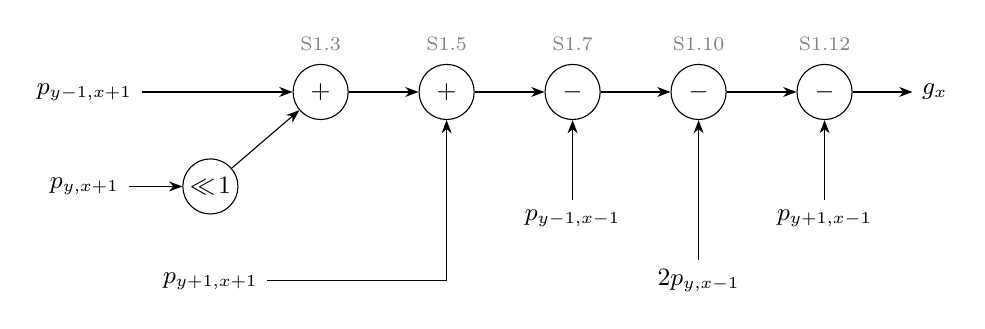
\begin{tikzpicture}[
  op/.style={draw, circle, minimum size=7mm, inner sep=0pt, font=\small},
  inp/.style={font=\small},
  note/.style={font=\scriptsize, text=gray},
  ->, >=Stealth]
  \node[inp] (a) at (0, 0) {$p_{y-1,x+1}$};
  \node[inp] (b) at (0, -1.2) {$p_{y,x+1}$};
  \node[op] (sh1) at (1.6, -1.2) {$\ll\!1$};
  \node[inp] (c) at (1.6, -2.4) {$p_{y+1,x+1}$};
  \node[op] (s3) at (3.0, 0) {$+$};
  \node[op] (s5) at (4.6, 0) {$+$};
  \node[op] (s7) at (6.2, 0) {$-$};
  \node[op] (s10) at (7.8, 0) {$-$};
  \node[op] (s12) at (9.4, 0) {$-$};
  \node[inp] (gx) at (10.8, 0) {$g_x$};
  \node[note, above=0.5mm of s3] {S1.3};
  \node[note, above=0.5mm of s5] {S1.5};
  \node[note, above=0.5mm of s7] {S1.7};
  \node[note, above=0.5mm of s10] {S1.10};
  \node[note, above=0.5mm of s12] {S1.12};
  \node[inp] (d) at (6.2, -1.6) {$p_{y-1,x-1}$};
  \node[inp] (e) at (7.8, -2.4) {$2p_{y,x-1}$};
  \node[inp] (f) at (9.4, -1.6) {$p_{y+1,x-1}$};
  \draw (a) -- (s3); \draw (b) -- (sh1); \draw (sh1) -- (s3);
  \draw (s3) -- (s5); \draw (c) -| (s5);
  \draw (s5) -- (s7); \draw (d) -- (s7);
  \draw (s7) -- (s10); \draw (e) -- (s10);
  \draw (s10) -- (s12); \draw (f) -- (s12);
  \draw (s12) -- (gx);
\end{tikzpicture}
\caption{Part of the DFG of segment S1: the five approximable operations that compute $g_x$ (lines 12 and 13).
Then $|g_x|$ uses a comparison, the negation S1.23 and a selection; S1.28 adds $|g_x|$ and $|g_y|$; a shift by 2 and
a \texttt{min} produce the output pixel.}
\label{fig:dfg}
\end{figure}

\paragraph{Assignment.} An \emph{assignment} is a map $u : O \to \bigcup_i \mathcal{U}_i$ with
$u(o_i) \in \mathcal{U}_i$. The exact design is $u^\star$, with $u^\star(o_i) = u_i^\star$ for all $i$.

\paragraph{Error of a value.} For any value $v$ of the DFG, the error is the approximate value minus the exact one,
\[
  e_v = \tilde v - v .
\]
The static model keeps, for each value, the mean, the second moment and the variance of the error over all executions:
\[
  \mu_v = \E[e_v], \qquad m_v = \E[e_v^2], \qquad \sigma_v^2 = m_v - \mu_v^2 .
\]

\paragraph{Profile.} The kernel runs once with the exact units on the chosen input data. The run records the mean
$\E[v]$ and the mean square $\E[v^2]$ of every value, up to $S = 4096$ samples $(x_s, y_s)$ of the operands of each
operation, and up to $R = 2048$ complete executions of each segment.

\examplebox{profile}{The body of \texttt{cols} runs $190 \times 190 = 36100$ times on the test image. S1.3 gets 4096
pairs $(p_{y-1,x+1}, 2p_{y,x+1})$ taken from those executions, and segment S1 keeps 2048 executions with all their
intermediate values.}

%======================================================================================================================
\section{Cost model}\label{sec:cost}

\subsection{Scheduling}

Let $T_c$ be the clock period, $t_{cq}$ the clock to output time and $t_{su}$ the setup time of a register. Operations
are chained in one cycle while
\[
  \sum_{k \in \text{chain}} d_k \le T_c - t_{cq} - t_{su},
\]
where $d_k$ is the delay of the unit of operation $k$ (sky130 synthesis, or Vivado when the FPGA delays are chosen). An
operation with $d_k > T_c - t_{cq} - t_{su}$ is a multicycle operation that takes
$\lceil (d_k + t_{cq} + t_{su}) / T_c \rceil$ cycles.

For a pipelined loop with requested interval $II_{\text{req}}$, the achieved interval is
\[
  II = \max\left( II_{\text{req}},\; \max_{r} \left\lceil \frac{U_r}{N_r} \right\rceil,\; II_{\text{rec}} \right),
\]
where $U_r$ is the number of uses of resource $r$ per iteration (memory bank ports, or units limited by
\texttt{allocation}), $N_r$ the number of instances (or ports) of $r$, and $II_{\text{rec}}$ the smallest interval that
satisfies every recurrence (the latency of the cycle of each loop carried value).

\examplebox{interval}{\texttt{in} is partitioned cyclically by 3 in its first dimension, so bank $b$ holds the rows
with $y \bmod 3 = b$. One iteration reads 3 pixels of row $y-1$, 2 of row $y$ (\texttt{in[y][x-1]} and
\texttt{in[y][x+1]}) and 3 of row $y+1$. These rows are in different banks, each with 2 ports, so
\[
  II = \max\big(1,\; \lceil 3/2 \rceil,\; \lceil 2/2 \rceil,\; \lceil 3/2 \rceil\big) = 2 .
\]
The simulator reports exactly this: \texttt{II 2 (mem: in (L1) mod 3)}. Sobel has no recurrence, so
$II_{\text{rec}}$ does not limit it.}

The latency of a pipelined loop with $N$ iterations and depth $D$ (cycles of one iteration) is
\[
  L_{\text{pipe}} = D + (N - 1)\, II + \ell_{\text{pipe}},
\]
and of a sequential loop with body latency $L_b$ and $s$ inner loops
\[
  L_{\text{seq}} = N \left( L_b + \ell_{\text{loop}} + s\, \ell_{\text{sub}} + \ell_{\text{addr}} \right),
\]
with the constants $\ell_{\text{pipe}} = 1$, $\ell_{\text{loop}} = 1$ and $\ell_{\text{sub}} = 2$ calibrated against
Vitis HLS, and $\ell_{\text{addr}}$ the latency of the bank remainder when the partition factor is not a power of 2.
A sequential loop whose only body is a pipelined loop is flattened into one loop of $N_{\text{out}} N_{\text{in}}$
iterations, as Vitis HLS does.

\examplebox{latency}{\texttt{rows} contains only the pipelined \texttt{cols}, so both are flattened into one loop of
$N = 190 \times 190 = 36100$ iterations. The depth of one iteration is $D = 18$ cycles (the bank remainder by 3, the
loads, the adder chains and the output). Then
\[
  L = 18 + (36100 - 1) \cdot 2 + 1 = 72217 \text{ cycles} = 361.1\ \mu\text{s at } 5\text{ ns}.
\]}

\subsection{Units in context}\label{sec:context}

\paragraph{Constant propagation.} Each instance of a unit is costed with the bits of its inputs that are known: constant
operands, and high bits that the range proves to be zero or copies of the sign. Let $\phi_g(u, K)$ and $\phi_c(u, K)$
be the fractions of gates and of carry chain cells of the netlist of $u$ that remain live under the known bits $K$.
Then
\begin{gather*}
  A(u, K) = \phi_g(u, K)\, A(u), \qquad \text{LUT}(u, K) = \phi_g(u, K)\, \text{LUT}(u), \\
  \text{CARRY4}(u, K) = \phi_c(u, K)\, \text{CARRY4}(u).
\end{gather*}

\examplebox{units in context}{Alone, the exact 16 bit adder of the library has $A = 730.7\ \mu\text{m}^2$ and 16 LUTs.
In Sobel, the 13 instances together cost $4811\ \mu\text{m}^2$ and 105 LUTs, that is, $370\ \mu\text{m}^2$ and about 8
LUTs per instance ($\phi_g \approx 0.5$): the gates that depend only on known high bits are removed. This is why the
saving of an approximate unit is measured in context: removing low bits saves a larger fraction of what is left.}

\paragraph{Exact multiplication by a constant.} A product $x \cdot c$ with $x$ of $w$ bits is a sum of shifts. With
$d(c)$ the smaller number of nonzero digits between the binary and the canonical signed digit forms of $|c|$,
\[
  \text{LUT}(x \cdot c) = (d(c) - 1)(w + 1), \qquad
  \text{delay}(x \cdot c) = \lceil \log_2 d(c) \rceil \, d_{\text{add}} .
\]

\examplebox{constant multiplication}{In Sobel, $c = 2$ has $d(2) = 1$: the product is a wire, with no LUT and no
delay. In the sharpening kernel of the simulator, $5 \cdot p$ with $p$ of 8 bits has $5 = 101_2$, $d(5) = 2$, so it
costs $(2 - 1)(8 + 1) = 9$ LUTs and the delay of one adder: $p + (p \ll 2)$.}

\paragraph{Truncated adders.} An adder of $W$ bits truncated in $k$ bits computes
\[
  \text{TRUNC}_k(a, b) = \Big( \big\lfloor a / 2^k \big\rfloor + \big\lfloor b / 2^k \big\rfloor \Big)\, 2^k ,
\]
which is an exact adder of $W - k$ bits plus wires (the $k$ low output bits are zero). Logic synthesis does not always
find that structure, so the cost used is
\[
  q(\text{TRUNC}_k) = \min\left( q_{\text{synth}}(\text{TRUNC}_k),\; \frac{W - k}{W}\, q(\text{exact}_W) \right),
  \qquad q \in \{ A, E, P_{\text{leak}}, \text{LUT} \},
\]
and $\text{CARRY4}(\text{TRUNC}_k) \le \lceil (W - k)/4 \rceil$.

\examplebox{truncated adder}{For $W = 16$ and $k = 2$, the synthesis with minimum delay gave
$A = 753.2\ \mu\text{m}^2$, more than the exact adder ($730.7$). The structural bound is
$\tfrac{14}{16} \cdot 730.7 = 639.4\ \mu\text{m}^2$, so the model uses $639.4$. On FPGA the bound gives 14 LUTs and
$\lceil 14/4 \rceil = 4$ CARRY4. A truncated adder never costs more than the exact adder of the bits it keeps.}

\paragraph{Sharing.} Adders and multiplications by a constant have one unit per operation (exact or approximate). A
group $G$ of multiplications between variables that the schedule allows to share in $I$ instances is shared only if
\[
  \sum_{j=1}^{I} \left[ \kappa\big(u, K_j\big) + \sum_{s \in \{a,b\}} \kappa\big(\text{mux}(n_{j,s}, W)\big) \right]
  \;<\; \sum_{o \in G} \kappa\big(u, K_o\big),
\]
where $\kappa$ is the area (ASIC target) or LUT plus CARRY4 (FPGA target), $K_j$ the known bits common to the operations
bound to instance $j$, and $n_{j,s}$ the number of distinct sources at input $s$ of instance $j$. A multiplexer of $n$
inputs and $W$ bits costs $(n - 1)$ two input multiplexers per bit (ASIC) and $W \lceil (n-1)/3 \rceil$ LUTs (FPGA).
Sharing is decided per unit, so the rule is the same for exact and approximate units.

\examplebox{why adders are not shared}{On FPGA, a 16 bit adder costs 16 LUTs. Sharing two additions in one adder needs
a 2 input multiplexer of 16 bits at each input, $2 \times 16 \lceil 1/3 \rceil = 32$ LUTs, to save one adder of 16
LUTs. Sharing never pays for adders, so the 13 operations of Sobel always get 13 units, and an approximate unit in one
of them changes only that instance. For two 8 bit multiplications between variables, one shared multiplier costs
$101 + 2 \times 8 = 117$ LUTs against $2 \times 101 = 202$ LUTs for two, so sharing pays when the schedule allows it.}

\paragraph{Registers.} A value produced in cycle $c_p$ and last used in cycle $c_\ell$ needs registers for
$s = c_\ell - c_p$ stages; with pipelining each stage is a register of the width of the value. On FPGA, a chain of
$s \ge 3$ stages of $b$ bits becomes a shift register: $b \lceil (s - 1)/32 \rceil$ LUTs plus $b$ output flip flops.

\paragraph{Memory addressing.} With cyclic partitioning by a factor $F$ that is not a power of 2, each index needs a
division by a constant ($6w$ LUTs for $w$ bits) and a remainder whose latency $w + 4$ cycles enters the depth.

\paragraph{Energy per execution.}
\[
  E = \sum_{o} N_o\, E\big(u(o), K_o\big) \;+\; B_{\text{reg}}\, E_{\text{reg}}\, N_{\text{cyc}}
      \;+\; E_{\text{ctrl}} N_{\text{cyc}} \;+\; \Big( \sum_{\text{inst}} P_{\text{leak}} + B_{\text{reg}} P_{\text{leak,reg}} \Big) t_{\text{exec}},
\]
with $N_o$ the number of executions of operation $o$, $B_{\text{reg}}$ the register bits and $N_{\text{cyc}}$ the
cycles of the kernel. The unit energy $E(u, K)$ is the one of the library (uniform operands), scaled by the live
fraction, as the area.

\examplebox{cost of the exact Sobel}{Area $11662\ \mu\text{m}^2$ (units 4811, other cells 2346, registers 3603,
control 901, no multiplexer); 660 LUTs, 43 CARRY4 and 460 FF on FPGA; $1.165\ \mu\text{J}$ per image, of which
$0.343\ \mu\text{J}$ are the 13 adders ($13 \times 36100$ executions) and $0.725\ \mu\text{J}$ the registers. Replacing
only S1.3 by $\text{TRUNC}_2$ gives $11568\ \mu\text{m}^2$, 658 LUTs and 42 CARRY4: one approximate operation saves
little, so the search must change many of them.}

%======================================================================================================================
\section{Error metrics}

For an output array with $N$ written positions and peak value $P$ (the maximum of its type),
\[
  \text{ME} = \frac{1}{N} \sum_{j} e_j, \qquad
  \text{MSE} = \frac{1}{N} \sum_{j} e_j^2, \qquad
  \text{PSNR} = 10 \log_{10} \frac{P^2}{\text{MSE}} .
\]
SSIM (Wang et al., 2004) uses an $11 \times 11$ Gaussian window with $\sigma = 1.5$, normalized, only at positions where
the window fits, with $C_1 = (0.01 L)^2$, $C_2 = (0.03 L)^2$ and $L = 255$:
\[
  \text{SSIM}(X, Y) = \frac{1}{|\Omega|} \sum_{p \in \Omega}
  \frac{(2 \mu_x \mu_y + C_1)(2 \sigma_{xy} + C_2)}{(\mu_x^2 + \mu_y^2 + C_1)(\sigma_x^2 + \sigma_y^2 + C_2)},
\]
where the local moments are the window weighted means at position $p$.

\examplebox{PSNR constraint}{\texttt{out} is \texttt{u8}, so $P = 255$ and $P^2 = 65025$. A constraint
$\text{PSNR} \ge 40$~dB is the same as $\text{MSE} \le 65025 / 10^{4} = 6.50$. With only S1.3 in $\text{TRUNC}_2$,
the simulator estimates $\text{MSE} = 0.614$, so $\text{PSNR} = 10 \log_{10}(65025 / 0.614) = 50.2$~dB; the bit by
bit execution measures $0.632$ and $50.1$~dB.}

%======================================================================================================================
\section{Static error model}\label{sec:err}

The error model answers, for any assignment, ``what are $\mu$ and $m$ at each output?'' in milliseconds, without
running the approximate kernel. It has two parts: the error that each approximate unit adds (its \emph{own} error),
and how errors travel through the DFG to the outputs (the \emph{propagation}).

\subsection{Own error of a unit}

For an operation $o$ with exact result $x \circ y$ and unit function $f_u$, over the $S$ operand samples
$(x_s, y_s)$ of the profile,
\[
  \mu_o^{\text{own}} = \frac{1}{S} \sum_{s} \big( f_u(x_s, y_s) - x_s \circ y_s \big), \qquad
  m_o^{\text{own}} = \frac{1}{S} \sum_{s} \big( f_u(x_s, y_s) - x_s \circ y_s \big)^2 .
\]
The own error is added to the error that arrives at the operation as an independent term:
$\mu = \mu_{\text{prop}} + \mu^{\text{own}}$, $\sigma^2 = \sigma^2_{\text{prop}} + \sigma^{2,\text{own}}$.
Measuring on the real operands matters because the error of most approximate units depends on the operand values.

\examplebox{own error of a truncated adder}{For $\text{TRUNC}_k$ the error is
\[
  f_u(a, b) - (a + b) = -\big( (a \bmod 2^k) + (b \bmod 2^k) \big) \in \big[ -2(2^k - 1),\ 0 \big].
\]
In S1.3, $a = p_{y-1,x+1}$ and $b = 2p_{y,x+1}$, which is always even.
\begin{itemize}
  \item $k = 1$: $b \bmod 2 = 0$ and $a \bmod 2$ is 0 or 1 with about the same frequency, so $\mu \approx -0.5$ and
    $m \approx 0.5$. The profile gives $m^{\text{own}} = 0.45$.
  \item $k = 2$: $\alpha = a \bmod 4$ is about uniform in $\{0,1,2,3\}$ ($\E[\alpha] = 1.5$, $\E[\alpha^2] = 3.5$)
    and $\beta = b \bmod 4 \in \{0, 2\}$ ($\E[\beta] = 1$, $\E[\beta^2] = 2$). If they are independent,
    $\mu = -(1.5 + 1) = -2.5$ and $m = 3.5 + 2 + 2 \cdot 1.5 \cdot 1 = 8.5$. The profile gives
    $\mu^{\text{own}} = -2.37$ and $m^{\text{own}} = 8.15$: real pixels are not uniform in their low bits.
\end{itemize}}

\subsection{Subtraction and signed addition}

In two's complement with $W$ bits, signed and unsigned additions are the same modulo $2^W$, and
\[
  a - b \equiv \overline{\,\overline{a} + b\,} \pmod{2^W}, \qquad \overline{x} = 2^W - 1 - x,
\]
since $\overline{\overline{a} + b} = 2^W - 1 - (2^W - 1 - a + b) = a - b$. An approximate subtraction is therefore
$\overline{f_u(\overline{a}, b)}$, with no carry in, and the result is read in the bits of the type of the node. An
operation stays exact when its result does not fit the $W$ bits of the unit. In hardware the inversions are free (an
inverter merges into the first gate or LUT), so the exact subtraction keeps the cost of the exact adder.

With $\text{TRUNC}_k$, let $r = (\overline{a} \bmod 2^k) + (b \bmod 2^k)$. Then
$f_u(\overline{a}, b) = \overline{a} + b - r$ and
\[
  \overline{f_u(\overline{a}, b)} = 2^W - 1 - (\overline{a} + b - r) = a - b + r ,
\]
so the error of a truncated subtraction is $+r \in [0, 2(2^k - 1)]$: positive, while the error of a truncated
addition is negative.

\examplebox{truncated subtraction, 8 bits for readability}{$a = 100$, $b = 37$, $k = 2$. Then
$\overline{a} = 255 - 100 = 155$ and
\[
  f_u(155, 37) = \big(\lfloor 155/4 \rfloor + \lfloor 37/4 \rfloor\big) \cdot 4 = (38 + 9) \cdot 4 = 188, \qquad
  \overline{188} = 255 - 188 = 67 .
\]
The exact result is $63$, so the error is $+4 = (155 \bmod 4) + (37 \bmod 4) = 3 + 1$. In Sobel the subtractions
S1.7 to S1.12 and S1.17 to S1.21 accept these units because their results ($[-1020, 1020]$, 11 bits) fit in 16 bits.
Truncated additions and subtractions in the same chain have errors of opposite signs, which partly cancel; the
search examples in Section~\ref{sec:search} show the effect.}

\subsection{Analytic propagation}

Errors are assumed independent of each other and of the signals, except when the same value enters twice.
\begin{align*}
  \text{add, sub:}\quad & e = e_a \pm e_b, &&
    \mu = \mu_a \pm \mu_b,\quad \sigma^2 = \sigma_a^2 + \sigma_b^2 \\
  \text{mul:}\quad & e = a e_b + b e_a + e_a e_b, &&
    \mu = \E[a]\mu_b + \E[b]\mu_a + \mu_a\mu_b \\
  & && m = \E[a^2] m_b + \E[b^2] m_a + m_a m_b + 2\E[a]\E[b]\mu_a\mu_b \\
  & && \qquad + 2\E[a]\mu_a m_b + 2\E[b]\mu_b m_a \\
  x \ll k:\quad & e = 2^k e_x, && \mu = 2^k \mu_x,\quad m = 4^k m_x \\
  x \gg k:\quad & && \mu = \mu_x / S,\quad
     \sigma^2 = \frac{\sigma_x^2}{S^2} + \E\!\left[ \frac{q}{S}\Big(1 - \frac{q}{S}\Big) \right] \\
  & && \text{with } S = 2^k,\; q = e \bmod S,\; e \sim \mathcal{N}(\mu_x, \sigma_x^2) \\
  x \bmod 2^k:\quad & && \mu = 0,\quad m = \E\big[ q (S - q) \big]
\end{align*}
The second term of the right shift is the variance added by the rounding toward minus infinity: an error that is not
a multiple of $S$ sometimes changes the quotient and sometimes does not, depending on the low bits of the exact value.

\paragraph{Comparison.} For $c = (a \bowtie b)$, the error of the difference $\delta = a - b$ is
$e_\delta \sim \mathcal{N}(\mu_a - \mu_b, \sigma_a^2 + \sigma_b^2)$. For each sample with exact difference $d_s$ and exact
outcome $c_s$, the probability that the approximate comparison is true is, for example for $<$,
\[
  \pi_s = \Pr[d_s + e_\delta \le -1] = \Phi\!\left( \frac{-1 + 0.5 - d_s - \mu_\delta}{\sigma_\delta} \right),
\]
and analogously for $\le$, $>$, $\ge$, $=$, $\ne$. Then
$\mu_c = \frac{1}{S}\sum_s (\pi_s - c_s)$ and $m_c = \frac{1}{S}\sum_s \Pr[\text{outcome changes}]$.

\paragraph{Selection.} For $y = c\,?\,A : B$ with flip probability $p_s$ (as above), chosen side error $e_{\text{ch}}$,
other side error $e_{\text{ot}}$ and exact distance $D_s$ between the sides,
\[
  \mu_y = \frac{1}{S}\sum_s \Big[ (1 - p_s)\mu_{\text{ch}} + p_s (D_s + \mu_{\text{ot}}) \Big], \quad
  m_y = \frac{1}{S}\sum_s \Big[ (1 - p_s) m_{\text{ch}} + p_s (D_s^2 + 2 D_s \mu_{\text{ot}} + m_{\text{ot}}) \Big].
\]
This covers \texttt{min}, \texttt{max}, \texttt{abs} and the conditional operator.

\examplebox{from S1.3 to the output, by hand}{Take only S1.3 in $\text{TRUNC}_2$: $\mu = -2.37$, $m = 8.15$
($\sigma^2 = 8.15 - 2.37^2 = 2.53$).
\begin{enumerate}
  \item S1.5 to S1.12 are exact and their other operands have no error, so by the add/sub rule the error of $g_x$ is
    the same: $\mu_{g_x} = -2.37$, $m_{g_x} = 8.15$.
  \item $|g_x| = (g_x < 0)\ ?\ (0 - g_x) : g_x$. The comparison flips only when $|g_x| \le 6$, which is rare, so
    $p_s \approx 0$. The chosen side has error $+e$ when $g_x \ge 0$ and $-e$ when $g_x < 0$: the second moment stays
    $8.15$, and the mean becomes $-2.37\,(\Pr[g_x \ge 0] - \Pr[g_x < 0])$, close to zero for edges in both directions.
  \item S1.28 adds $|g_y|$, which has no error: $m = 8.15$.
  \item The shift by 2 ($S = 4$) divides the second moment by 16 and adds the rounding term. The error
    $\pm(\alpha + \beta)$ modulo 4 is 0 with probability $2/8$, 2 with $2/8$, and 1 or 3 with $4/8$, so
    $\E[\tfrac{q}{4}(1 - \tfrac{q}{4})] = \tfrac{2}{8}\cdot\tfrac{1}{4} + \tfrac{4}{8}\cdot\tfrac{3}{16} = 0.156$.
    Then $m_{\text{out}} \approx 8.15/16 + 0.156 = 0.67$.
  \item \texttt{min(255, ...)} rarely saturates, so it changes almost nothing.
\end{enumerate}
The hand estimate, $0.67$ ($49.9$~dB), is close to the simulator's estimate, $0.614$, and to the measured value,
$0.632$. The simulator is closer because its default model, next, keeps the correlation between the error and the low
bits of the exact sum.}

\subsection{Sampled propagation}

Inside each segment, the $R$ stored exact executions are replayed with the approximate units. Values that enter the
segment from other segments, recurrences or memory get a noise $\lfloor \mathcal{N}(\mu, \sigma^2) + U(0,1) \rfloor$
with their propagated moments. For each node,
\[
  \mu_v = \frac{1}{R} \sum_{r} (\tilde v_r - v_r), \qquad m_v = \frac{1}{R} \sum_{r} (\tilde v_r - v_r)^2 .
\]
Correlations inside the segment (an adder that already cleared the low bits of several terms, errors that depend on the
low bits of the operands, the sign of $g_x$ in \texttt{abs}) are kept. This is the default model.

\examplebox{sampled model}{In Sobel the whole body is one segment and the inputs come from memory with no error, so
the sampled model is the replay of 2048 real neighborhoods of $3 \times 3$ pixels with the approximate adders.
Nothing is assumed about independence inside the expression; the only approximation is that 2048 neighborhoods
represent the 36100 of the image.}

\subsection{Recurrences}

For a loop carried value with $T$ iterations, the increment per iteration $\delta = (\mu_\delta, \sigma_\delta^2)$ is
measured with no input error, and the gain $g$ with the analytic model by a probe of size $p$:
\[
  g = \frac{\mu_{\text{out}}(p) - \mu_{\text{out}}(0)}{p}, \qquad
  \mu_{t+1} = g\,\mu_t + \mu_\delta, \qquad \sigma^2_{t+1} = g^2 \sigma^2_t + \sigma^2_\delta .
\]
Uses inside the loop see the average over the iterations,
$\bar\mu = \frac{1}{T}\sum_t \mu_t$, $\bar m = \frac{1}{T}\sum_t (\sigma_t^2 + \mu_t^2)$; uses after the loop see
$(\mu_T, \sigma_T^2)$.

\examplebox{accumulation}{Sobel has no recurrence. In the dot product kernel, \texttt{acc += a[i] * b[i]} has gain
$g = 1$, so after $T$ iterations $\mu_T = T \mu_\delta$ and $\sigma_T^2 = T \sigma_\delta^2$: the bias of a multiplier
grows with $T$, while its random part grows only with $\sqrt{T}$ in standard deviation. Over 1024 products, a small
bias dominates.}

\subsection{Memory}

Each array keeps the mean of the errors written to it, weighted by the number of executions $w$ of each store:
\[
  \mu_{\text{arr}} = \frac{\sum w\, \mu}{\sum w}, \qquad m_{\text{arr}} = \frac{\sum w\, m}{\sum w}.
\]
Loads see $(\mu_{\text{arr}}, m_{\text{arr}})$; outputs give $\text{ME} = \mu$, $\text{MSE} = m$ and the PSNR.
In Sobel, \texttt{out} has one store, so its ME and MSE are the moments of that store.

\subsection{SSIM estimate}

Let $\mu_x, \sigma_x^2$ be the local moments of the exact image (computed once). With the error independent of the signal,
with mean $\mu_e$ and variance $\sigma_e^2$,
\[
  \mu_y = \mu_x + \mu_e, \qquad \sigma_y^2 = \sigma_x^2 + \sigma_e^2, \qquad \sigma_{xy} = \sigma_x^2 .
\]
With a part proportional to the value, $e = a + b\,x + n$, $b = \operatorname{Cov}(x, e)/\Var(x)$,
$a = \mu_e - b\,\E[x]$, $\sigma_n^2 = \max(0, \sigma_e^2 - b^2 \Var(x))$:
\[
  \mu_y = (1+b)\mu_x + a, \qquad \sigma_y^2 = (1+b)^2\sigma_x^2 + \sigma_n^2, \qquad \sigma_{xy} = (1+b)\sigma_x^2 .
\]
With the error conditioned on the exact value (sampled model), in $B = 32$ value bins with mean $m_\beta$ and variance
$v_\beta$, and the blurred indicator maps $P_\beta = G * \mathbb{1}[x \in \beta]$ and $Q_\beta = G * (x\,\mathbb{1}[x \in \beta])$:
\begin{gather*}
  \mu_y = \mu_x + \sum_\beta m_\beta P_\beta, \qquad
  \E[xy] = \E[x^2] + \sum_\beta m_\beta Q_\beta, \\
  \E[y^2] = \E[x^2] + 2\sum_\beta m_\beta Q_\beta + \sum_\beta (m_\beta^2 + v_\beta) P_\beta,
\end{gather*}
and the local SSIM follows from these moments. All three assume errors independent between pixels.

\examplebox{limit of the SSIM estimate}{In Sobel, neighboring output pixels share 6 of their 9 input pixels, so their
errors are correlated: the errors form small structures in the image, which SSIM penalizes more than independent
noise of the same MSE. For this reason the SSIM estimate is optimistic on Sobel (in the results of
Table~\ref{tab:sobel}, 0.95 estimated against 0.92 measured), and the verification step (Section~\ref{sec:verify}) is
what guarantees an SSIM constraint.}

%======================================================================================================================
\section{Search}\label{sec:search}

\subsection{Problem}

Given an objective $\Cost(u)$ (area, LUT plus CARRY4, energy, latency, interval, or a weighted sum normalized by the
exact design) and an error constraint on every output $k$ (PSNR $\ge \tau$, MSE $\le \tau$ or SSIM $\ge \tau$), the
problem is
\[
  \min_{u} \; \Cost(u) \quad \text{subject to} \quad \Feas(u) = \bigwedge_k \text{constraint}\big(\hat E_k(u)\big),
\]
where $\hat E_k$ is the static estimate of output $k$. The directives (pipeline, unroll, partitioning) and the clock
are the ones of the code and of the page; the search changes only the units.

The page offers six heuristics, described below in this order: two constructive ones, sequential and efficiency, and
four improvement ones, local search (the default), tabu search, GRASP and a genetic algorithm. The option ``all''
runs the six and draws their fronts in the same chart.

\paragraph{Groups.} The operations are partitioned into groups $\mathcal{G}$, and all operations of a group get the
same unit, so the decision is a vector $\mathbf{c} \in \prod_{g} \mathcal{C}_g$ with one candidate unit per group.
There are two granularities:
\begin{itemize}
  \item \textbf{per operation}: each operation is a group; this is the finest decision, and the only one that can
    give different units to the copies of an unrolled operation;
  \item \textbf{per line}: the operations with the same source line, operation and width form a group; this is what a
    designer changes when editing the code, and it gives a much smaller search space.
\end{itemize}

\examplebox{groups of Sobel}{Per operation, there are 13 groups. Per line, there are 6:
\begin{center}
\rowcolors{2}{gray!10}{white}
\begin{tabular}{|l|l|r|l|}
\hline
\rowcolor{tabAzul}\color{white} Group & \color{white} Operations & \color{white} Candidates & \color{white} Note \\
\hline
line 12, add & S1.3, S1.5 & 13 & $g_x$, positive terms \\
line 13, sub & S1.7, S1.10, S1.12 & 17 & $g_x$, negative terms \\
line 14, add & S1.15, S1.16 & 14 & $g_y$, positive terms \\
line 15, sub & S1.17, S1.20, S1.21 & 13 & $g_y$, negative terms \\
line 16, sub & S1.23, S1.26 & 1 & negations, exact only \\
line 16, add & S1.28 & 14 & $|g_x| + |g_y|$ \\
\hline
\end{tabular}
\end{center}
The search space has $13 \cdot 17 \cdot 14 \cdot 13 \cdot 1 \cdot 14 = 563108$ points per line, and about
$4.7 \times 10^{12}$ per operation. With one synthesis and one error estimate per point (about 30~ms), even the
smaller space would take hours to enumerate, which is why the heuristics below exist.}

\paragraph{Scalar error.} To compare two infeasible points, or to measure how much error a move adds, the search uses
\[
  \varepsilon(u) = \sum_k \frac{\text{MSE}_k(u)}{P_k^2} \quad\text{(PSNR, MSE)}, \qquad
  \varepsilon(u) = \sum_k \big(1 - \text{SSIM}_k(u)\big) \quad\text{(SSIM)}.
\]

\paragraph{Cost is not additive.} Each evaluation synthesizes the whole design (scheduling, binding, sharing,
multiplexers, registers), so the cost of two changes is not the sum of the costs of each one. A unit with a longer
delay can, for example, add a pipeline stage and its registers, or a change of unit can let two multiplications share
an instance.

\subsection{Candidates of a group}

The library has dozens of units per width (Sobel has 96 for 16 bit adders). Most of them are useless in a given
group: they cost more, or err more for the same saving. Algorithm~\ref{alg:cand} keeps, per group, only the units on
the Pareto front of (saving in context, own error).

\begin{algorithm}[H]
\caption{Candidates of a group}\label{alg:cand}
\begin{algorithmic}[1]
\Require group $g$ with operations $O_g$, exact unit $u^\star_g$, exact design $u^\star$ of the whole kernel
\State $R \gets \{ (u^\star_g, 0, 0) \}$
\For{$u \in \bigcap_{o \in O_g} \mathcal{U}_o \setminus \{u^\star_g\}$}
  \State $\text{own} \gets \sum_{o \in O_g} m_o^{\text{own}}(u)$
  \If{$\text{own} = 0$} \textbf{continue} \Comment{same results as the exact unit on the real operands}
  \EndIf
  \State $\Delta \gets \Cost(u^\star[O_g \mapsto u]) - \Cost(u^\star)$ \Comment{saving in context, full synthesis}
  \If{$\Delta \ge 0$} \textbf{continue}
  \EndIf
  \State $R \gets R \cup \{(u, \Delta, \text{own})\}$
\EndFor
\State $\mathcal{C}_g \gets$ Pareto front of $R$ in $(\Delta, \text{own})$, exact unit first, then increasing own error
\State \Return $\mathcal{C}_g$
\end{algorithmic}
\end{algorithm}

\examplebox{candidates of S1.3, area objective}{The front starts like this ($\Delta$ in $\mu\text{m}^2$):
\begin{center}
\rowcolors{2}{gray!10}{white}
\begin{tabular}{|l|r|r|}
\hline
\rowcolor{tabAzul}\color{white} Unit & \color{white} $\Delta$ & \color{white} $m^{\text{own}}$ \\
\hline
ADD16 exact & 0 & 0 \\
ADD16 TRUNC1 & $-47$ & 0.45 \\
ADD16 LOA2 & $-67$ & 0.93 \\
ADD16 LOA3 & $-95$ & 3.99 \\
ADD16 LOA4 & $-131$ & 18.1 \\
ADD16 TRUNC3 & $-140$ & 55.2 \\
\hline
\end{tabular}
\end{center}
and continues up to $\text{TRUNC}_8$ ($-370$, $7.8 \times 10^4$): 14 candidates out of 96. $\text{TRUNC}_2$ is not on
the front of S1.3 because $\text{LOA}_3$ saves more with less error in this operation. Units whose split falls in the
high bits that are always zero (some segmented adders) have $\text{own} = 0$ and are removed: in context they are the
exact adder.}

Algorithm~\ref{alg:eval} is the only way the heuristics touch a design.

\begin{algorithm}[H]
\caption{Evaluate}\label{alg:eval}
\begin{algorithmic}[1]
\Require choice $\mathbf{c}$ (one unit per group)
\If{$\mathbf{c}$ is in the cache} \Return cached point
\EndIf
\State $u \gets$ expand $\mathbf{c}$ to the operations; synthesize; $\Cost \gets$ objective of the synthesis
\State $\hat E \gets$ static error estimate (own errors, propagation)
\State \Return $(\mathbf{c}, \Cost, \varepsilon, \Feas)$, stored in the cache and in the list of evaluated points
\end{algorithmic}
\end{algorithm}

A cheaper call, \textsc{CostOnly}$(\mathbf{c})$, runs only the synthesis. The heuristics use it to discard moves that
do not save anything before paying for the error estimate.

\subsection{Constructive heuristics}

They build one solution from the exact design, one decision at a time.

\paragraph{Sequential.} Algorithm~\ref{alg:seq} visits the groups once, multiplications first and then in source
order, and in each one keeps the cheapest candidate that leaves the design feasible. It is fast, but a decision is
never revisited.

\begin{algorithm}[H]
\caption{Sequential}\label{alg:seq}
\begin{algorithmic}[1]
\State $\mathbf{c} \gets \mathbf{c}^\star$ (all exact); order groups: multiplications first, then source order
\For{each group $g$ in that order}
  \State $\text{best} \gets \text{Evaluate}(\mathbf{c})$
  \For{$u \in \mathcal{C}_g$}
    \State $p \gets \text{Evaluate}(\mathbf{c}[g \mapsto u])$
    \If{$p$ feasible \textbf{and} $\Cost(p) < \Cost(\text{best})$} $\text{best} \gets p$
    \EndIf
  \EndFor
  \State $\mathbf{c} \gets \text{best}.\mathbf{c}$
\EndFor
\end{algorithmic}
\end{algorithm}

\examplebox{sequential on Sobel, per line, 40 dB}{
\begin{center}
\rowcolors{2}{gray!10}{white}
\begin{tabular}{|l|l|r|r|}
\hline
\rowcolor{tabAzul}\color{white} Step & \color{white} Choice & \color{white} Area ($\mu\text{m}^2$) & \color{white} PSNR (dB) \\
\hline
start & all exact & 11662 & $\infty$ \\
line 12 (add) & $\text{TRUNC}_3$ & 11381 & 40.39 \\
line 13 (sub) & $\text{TRUNC}_3$ & 10803 & 41.98 \\
line 14 (add) & $\text{LOA}_3$ & 10611 & 40.78 \\
line 15 (sub) & $\text{LOA}_3$ & 9965 & 41.58 \\
line 16 (add) & $\text{LOA}_7$ & 9722 & 40.56 \\
\hline
\end{tabular}
\end{center}
Line 12 alone takes almost the whole budget (40.39~dB). Then line 13 in $\text{TRUNC}_3$ \emph{raises} the PSNR to
41.98~dB: the positive error of the truncated subtractions cancels the negative error of the truncated additions of
the same line of $g_x$, exactly as in the subtraction example. The order of the code decides which lines get the
large truncations.}

\paragraph{Efficiency.} Algorithm~\ref{alg:eff} starts from the exact design and, at each step, applies the move with
the largest saving per unit of added error,
\[
  \rho(m) = \frac{\Delta C(m)}{\Delta \varepsilon(m)}, \qquad
  \Delta C = \Cost(\text{cur}) - \Cost(\mathbf{c} \oplus m), \quad
  \Delta\varepsilon = \varepsilon(\mathbf{c} \oplus m) - \varepsilon(\text{cur}),
\]
until no feasible move saves anything. A move $m = (g, u)$ changes one group to unit $u$; with groups finer than the
class, there are also moves that change every group of a class (all 16 bit additions, for example) to the same unit.
A move that saves with no added error gets $\rho = 10^{15} + \Delta C$, so it is always taken first.

\emph{Lazy evaluation.} Recomputing $\rho$ for every move at every step costs one evaluation per move. When there are
more than 400 moves, each move keeps the last $\rho$ computed for it, and a step recomputes only the moves with the
largest stored $\rho$ (at least 40) until the best recomputed value is not below the best stored one. This assumes
that the efficiency of a move does not grow when other moves are applied (diminishing returns), which holds
approximately; the moves of the group that changed are always recomputed.

\begin{algorithm}[H]
\caption{Efficiency (greedy by saving per error, lazy evaluation)}\label{alg:eff}
\begin{algorithmic}[1]
\State $\mathbf{c} \gets \mathbf{c}^\star$; $\text{cur} \gets \text{Evaluate}(\mathbf{c})$
\State moves $M \gets \{(g, u) : u \in \mathcal{C}_g\} \cup \{(\text{class } k, u)\}$
\State stored rate $\rho(m) \gets +\infty$ for all $m \in M$
\Loop
  \State recompute the moves with the largest stored $\rho$ (at least 40, all when $|M| \le 400$) until the best
  fresh rate is not below the best stored one
  \For{each recomputed move $m$}
    \State $\Delta C \gets \Cost(\text{cur}) - \textsc{CostOnly}(\mathbf{c} \oplus m)$
    \If{$\Delta C \le 0$} discard $m$; \textbf{continue}
    \EndIf
    \State $p \gets \text{Evaluate}(\mathbf{c} \oplus m)$; \; $\Delta\varepsilon \gets \varepsilon(p) - \varepsilon(\text{cur})$
    \If{$p$ infeasible} discard $m$; \textbf{continue}
    \EndIf
    \State $\rho(m) \gets \Delta C / \Delta\varepsilon$ \; (or $10^{15} + \Delta C$ when $\Delta\varepsilon \le 0$)
  \EndFor
  \If{no feasible saving move} \textbf{break}
  \EndIf
  \State apply the move with the largest $\rho$; reset $\rho$ of the moves of the changed groups to $+\infty$
\EndLoop
\end{algorithmic}
\end{algorithm}

\examplebox{efficiency on Sobel, per line, 40 dB}{The 17 steps go up the candidate lists of all lines at the same
pace. The first ones:
\begin{center}
\rowcolors{2}{gray!10}{white}
\begin{tabular}{|r|l|r|r|r|}
\hline
\rowcolor{tabAzul}\color{white} Step & \color{white} Move & \color{white} $\Delta C$ & \color{white} $\Delta\varepsilon$ & \color{white} PSNR (dB) \\
\hline
1 & line 15 (sub) $\to \text{TRUNC}_1$ & 299 & $3.8 \times 10^{-6}$ & 54.21 \\
2 & line 14 (add) $\to \text{TRUNC}_1$ & 93 & $-0.5 \times 10^{-6}$ & 54.88 \\
3 & line 13 (sub) $\to \text{TRUNC}_1$ & 479 & $3.1 \times 10^{-6}$ & 51.98 \\
4 & line 12 (add) $\to \text{TRUNC}_1$ & 93 & $-1.7 \times 10^{-6}$ & 53.32 \\
5 & line 16 (add) $\to \text{LOA}_2$ & 73 & $2.2 \times 10^{-6}$ & 51.65 \\
\hline
\end{tabular}
\end{center}
Steps 2 and 4 save area \emph{and} reduce the error ($\Delta\varepsilon < 0$, $\rho = 10^{15} + \Delta C$): the
truncated addition cancels part of the error of the truncated subtraction of the same component. The search ends at
step 17 with $9820\ \mu\text{m}^2$ (15.8\% less area) and 40.25~dB, with lines 12 and 14 in $\text{LOA}_4$, lines 13
and 15 in $\text{LOA}_3$ and line 16 in $\text{LOA}_6$. Every remaining single move violates the constraint. Note
that sequential, with a cruder rule, ended cheaper (9722): small steps with the best ratio do not lead to the large
truncations that cancel each other.}

\subsection{Starting points of the improvement heuristics}

All improvement heuristics start from several points and keep the cheapest feasible result, so they never end worse
than any starting point. The points are (Algorithm~\ref{alg:seed}): the exact design, the result of efficiency, and
the \emph{class optimum} carried to the groups. The class optimum uses one unit per class and width (one unit for all
the 16 bit additions of Sobel, for example). With one group per class the space is small, so it is solved exactly:
every combination is costed with \textsc{CostOnly}, sorted by cost, and the error is evaluated in that order; the first
feasible combination is the optimum among the class candidates. This enumeration is internal to the starting points;
it is not offered as a heuristic, because per operation or per line the space is too large for it.

\begin{algorithm}[H]
\caption{Starting points}\label{alg:seed}
\begin{algorithmic}[1]
\State $S \gets \{ \text{Evaluate}(\mathbf{c}^\star) \}$
\State $\mathcal{K} \gets$ class groups (one per operation class and width) with their candidates
\If{$\prod_{k \in \mathcal{K}} |\mathcal{C}_k| \le 20000$}
  \State cost every combination of $\prod_k \mathcal{C}_k$ with \textsc{CostOnly}; sort by cost
  \State $\mathbf{k} \gets$ first combination, in that order, whose Evaluate is feasible
  \State $\mathbf{c} \gets$ for each group, the unit of its class in $\mathbf{k}$ (exact if its operations disagree)
  \State $S \gets S \cup \{\text{Evaluate}(\mathbf{c})\}$
\EndIf
\State $S \gets S \cup \{\text{Evaluate}(\text{Efficiency result})\}$
\State \Return the distinct feasible points of $S$, cheapest first
\end{algorithmic}
\end{algorithm}

\examplebox{class optimum of Sobel}{All 13 operations are 16 bit additions or subtractions, so there is a single class
group with 11 candidates (from $\text{LOA}_2$, saving $568\ \mu\text{m}^2$ with all 13 operations, up to
$\text{TRUNC}_{16}$). The enumeration evaluates at most 11 points and gives the best single unit for the whole kernel.
Carried to the 6 line groups, it becomes a starting point in which every line uses that unit (the negations stay
exact).}

\subsection{Improvement heuristics}

\paragraph{Local search with pair moves.} Algorithm~\ref{alg:ls} is the core of the improvement heuristics. From the
current point it tries the single group moves that reduce the cost, in increasing cost, and takes the first feasible
one. When every such move is infeasible, it tries \emph{pairs}: a move that saves but violates the constraint,
combined with a move in another group to a unit with less own error. The pair can be feasible and still cheaper than
the current point: it moves error budget from a group where it saves little to one where it saves more. The search
stops when neither single moves nor pairs improve, or when the evaluation budget ends.

\begin{algorithm}[H]
\caption{Local search with pair moves}\label{alg:ls}
\begin{algorithmic}[1]
\Require start point $\text{cur}$, evaluation budget
\Loop
  \State $D \gets \{ \mathbf{c} = \text{cur}.\mathbf{c}[g \mapsto u] : u \in \mathcal{C}_g \cup \{u_g^\star\},\; \textsc{CostOnly}(\mathbf{c}) < \Cost(\text{cur}) \}$, sorted by cost
  \State $\text{next} \gets$ first feasible $\text{Evaluate}(\mathbf{c})$, $\mathbf{c} \in D$
  \If{$\text{next} = \emptyset$}
    \State $D' \gets \emptyset$
    \For{$m$ among the 12 cheapest evaluated moves of $D$ (all infeasible)}
      \For{each other group $h$ and unit $w$ with own error below that of $m.\mathbf{c}[h]$}
        \State $\mathbf{c}' \gets m.\mathbf{c}[h \mapsto w]$; add it to $D'$ if $\textsc{CostOnly}(\mathbf{c}') < \Cost(\text{cur})$
      \EndFor
    \EndFor
    \State $\text{next} \gets$ first feasible $\text{Evaluate}(\mathbf{c}')$, $\mathbf{c}' \in D'$ in increasing cost
  \EndIf
  \If{$\text{next} = \emptyset$ \textbf{or} budget exhausted} \textbf{break}
  \EndIf
  \State $\text{cur} \gets \text{next}$
\EndLoop
\State \Return $\text{cur}$
\end{algorithmic}
\end{algorithm}

\begin{algorithm}[H]
\caption{Local (the default heuristic of the page)}\label{alg:local}
\begin{algorithmic}[1]
\State \Return the cheapest of LocalSearch$(s)$ over the starting points $s$
\end{algorithmic}
\end{algorithm}

\examplebox{local search on Sobel, per line, 40 dB}{The two starting points are the efficiency result
($9820\ \mu\text{m}^2$) and the class optimum. From the class optimum, a chain of pair moves (line 16 back to exact
with line 12 in $\text{LOA}_4$, then line 16 in $\text{LOA}_7$, and so on) ends at $9851\ \mu\text{m}^2$. From the
efficiency result, every single move and every pair is infeasible or more expensive, so it is a local optimum of this
neighborhood. The answer is $9820\ \mu\text{m}^2$. A pair changes two groups, and only toward less own error in the
second group; the cheaper point of Table~\ref{tab:sobel} found by hand differs from the efficiency result in four
groups, all toward more own error, so it is outside this neighborhood.}

\paragraph{Tabu search.} Algorithm~\ref{alg:tabu} lets the search move to more expensive or infeasible points, to
leave a local optimum. A group that has just changed becomes \emph{tabu} for $\theta$ iterations (it cannot change
again), unless the move gives a point cheaper than the best found (aspiration). The best feasible point of each run
is polished by the local search.

\begin{algorithm}[H]
\caption{Tabu search}\label{alg:tabu}
\begin{algorithmic}[1]
\For{each starting point $s$}
  \State $\text{cur} \gets s$, $\text{run} \gets s$, tabu$(g) \gets 0$ for all groups
  \For{$t = 1, \dots, 40$}
    \State neighbors: all single group moves of $\text{cur}$ (cheaper or more expensive), sorted by cost
    \State evaluate the 16 cheapest that are not tabu ($\text{tabu}(g) < t$), or tabu but cheaper than the best so far
    \State $\text{cur} \gets$ cheapest feasible evaluated neighbor, or, with none feasible, the one with least error
    \State $\text{tabu}(g_{\text{moved}}) \gets t + \theta$, \; $\theta = \min(7, \max(3, \lceil |\mathcal{G}|/3 \rceil))$
    \If{$\text{cur}$ feasible \textbf{and} cheaper than $\text{run}$} $\text{run} \gets \text{cur}$
    \EndIf
  \EndFor
  \State $\text{run} \gets \text{LocalSearch}(\text{run})$
\EndFor
\State \Return the cheapest $\text{run}$
\end{algorithmic}
\end{algorithm}

\examplebox{tabu tenure}{Per line, Sobel has $|\mathcal{G}| = 6$, so $\theta = \min(7, \max(3, 2)) = 3$: a line that
changed waits 3 iterations. Per operation, $|\mathcal{G}| = 13$ and $\theta = \min(7, \max(3, 5)) = 5$.}

\paragraph{GRASP.} Algorithm~\ref{alg:grasp} (greedy randomized adaptive search procedure) builds several different
solutions with a randomized greedy and improves each one with the local search. In the construction, each group
chooses at random among the $\alpha$ cheapest feasible moves (the restricted candidate list, RCL), so each
construction ends in a different region of the space.

\begin{algorithm}[H]
\caption{GRASP}\label{alg:grasp}
\begin{algorithmic}[1]
\State $\text{best} \gets$ cheapest of LocalSearch$(s)$ over the starting points
\For{$i = 1, \dots, 6$}
  \State $\mathbf{c} \gets \mathbf{c}^\star$; shuffle the groups (fixed seed)
  \For{each group $g$ in that order}
    \State $\text{RCL} \gets$ the first $\alpha = 3$ feasible moves among the saving moves of $g$, in cost order
    \If{$\text{RCL} \ne \emptyset$} $\mathbf{c} \gets$ a uniform element of RCL
    \EndIf
  \EndFor
  \State $p \gets \text{LocalSearch}(\text{Evaluate}(\mathbf{c}))$; keep the cheapest feasible
\EndFor
\end{algorithmic}
\end{algorithm}

\examplebox{GRASP on Sobel, per line, 40 dB}{One of the randomized constructions visits the lines of $g_y$ early and
gives both of them $\text{TRUNC}_3$; the local search then completes it. The result, $9691\ \mu\text{m}^2$ (16.9\%)
at 40.53~dB, has lines 14 and 15 in $\text{TRUNC}_3$, lines 12 and 13 in $\text{LOA}_4$ and $\text{LOA}_3$, and line
16 in $\text{LOA}_6$: the pair of truncated lines whose errors cancel, now in $g_y$ instead of $g_x$.}

\paragraph{Genetic algorithm.} Algorithm~\ref{alg:ga} keeps a population of choices, one gene per group (the unit of
the group). Feasible points always rank above infeasible ones; among feasible points the cheaper wins, and among
infeasible ones the one with less error. Crossover mixes the units of two parents, and mutation changes a gene to a
random candidate.

\begin{algorithm}[H]
\caption{Genetic algorithm}\label{alg:ga}
\begin{algorithmic}[1]
\State population $P$: the starting points, the exact design, and mixes of a starting point and random genes
  (each gene from the start with probability $1/2$; a random gene is exact with probability $0.3$), size 24
\For{generation $= 1, \dots, 30$}
  \State $P' \gets$ the 2 best of $P$ (elitism), ranked by the feasibility rules
  \While{$|P'| < 24$}
    \State parents $a, b \gets$ binary tournaments with the same rules
    \State child: uniform crossover of $a.\mathbf{c}$ and $b.\mathbf{c}$; each gene mutated with probability $1/|\mathcal{G}|$
    \State $P' \gets P' \cup \{\text{Evaluate}(\text{child})\}$
  \EndWhile
  \State $P \gets P'$
\EndFor
\State \Return LocalSearch(cheapest feasible point found)
\end{algorithmic}
\end{algorithm}

\examplebox{one crossover per line}{Order the genes as lines 12, 13, 14, 15, 16 (sub) and 16 (add). Take as parent
$a$ the sequential result, (TRUNC3, TRUNC3, LOA3, LOA3, exact, LOA7), and as parent $b$ the GRASP result, (LOA4,
LOA3, TRUNC3, TRUNC3, exact, LOA6). A uniform crossover takes each gene from $a$ or $b$ with probability $1/2$.
\begin{itemize}
  \item The child (TRUNC3, TRUNC3, TRUNC3, TRUNC3, exact, LOA7) takes the truncated lines of both parents and the last
    gene of $a$. It costs $9521\ \mu\text{m}^2$ and its estimate is 40.29~dB, so it is feasible for the search, but
    the bit by bit execution measures 39.83~dB: the verification step rejects it.
  \item The child (TRUNC3, TRUNC3, TRUNC3, TRUNC3, exact, LOA6), the same with the last gene of $b$, costs
    $9562\ \mu\text{m}^2$ and measures 41.10~dB. It is the point found by hand in Table~\ref{tab:sobel}, cheaper than
    every heuristic result.
\end{itemize}
The second child comes from these parents with probability $2^{-5} = 1/32$ (gene 5 is the same in both). The GA of the
simulator does not start from these two parents, though: its population comes from the starting points (exact,
class optimum, efficiency), which have no truncated line, and a mutation (probability $1/6$ per gene with
$|\mathcal{G}| = 6$) must create each $\text{TRUNC}_3$ gene, so this child is possible but not likely in 30
generations.}

\subsection{Verification and result}\label{sec:verify}

The result of a heuristic is the cheapest feasible point among all the points it evaluated, not only the end of its
path. Since the static estimate has an error of its own, Algorithm~\ref{alg:verify} executes the best points bit by bit
before answering.

\begin{algorithm}[H]
\caption{Exploration driver}\label{alg:verify}
\begin{algorithmic}[1]
\State elaborate, profile (exact execution), build the groups and candidates
\For{each chosen heuristic $h$}
  \State run $h$; $F \gets$ feasible evaluated points sorted by cost
  \For{$p \in F$ (up to 25)}
    \State execute the approximate design bit by bit; measure the error of every output
    \If{the measured error satisfies the constraint} \Return $p$
    \EndIf
  \EndFor
\EndFor
\end{algorithmic}
\end{algorithm}

\examplebox{verification}{Suppose a heuristic had evaluated the point (TRUNC3, TRUNC3, TRUNC3, TRUNC3, exact, LOA7) of
the crossover example: $9521\ \mu\text{m}^2$, estimated 40.29~dB. It would be the first point of $F$. The bit by bit
execution measures 39.83~dB, below the constraint, so the driver goes to the next feasible point in cost order. The
estimate is 0.46~dB optimistic here because a margin of 0.29~dB is smaller than the error of the estimate itself; on
the points of Table~\ref{tab:sobel} the difference between estimate and measurement is at most 0.3~dB in PSNR.}

%======================================================================================================================
\section{Results on Sobel}\label{sec:results}

Table~\ref{tab:sobel} puts the pieces together: the six heuristics of the page on the Sobel kernel, area objective,
$\text{PSNR} \ge 40$~dB, 5~ns clock, sky130, test image of $192 \times 192$ pixels. The exact design has
$11662\ \mu\text{m}^2$. ``Est.'' is the static estimate used by the search and ``meas.'' the bit by bit execution;
the evaluations count the points that went through Evaluate (Algorithm~\ref{alg:eval}).

\begin{table}[h]
\centering
\small
\rowcolors{2}{gray!10}{white}
\begin{tabular}{|l|r|r|r|r|r|r|}
\hline
\rowcolor{tabAzul}\color{white} &
  \multicolumn{3}{c|}{\color{white} Groups per line (6)} &
  \multicolumn{3}{c|}{\color{white} Groups per operation (13)} \\
\rowcolor{tabAzul}\color{white} Heuristic & \color{white} Area ($\mu\text{m}^2$) & \color{white} PSNR est./meas. &
  \color{white} Evals & \color{white} Area ($\mu\text{m}^2$) & \color{white} PSNR est./meas. & \color{white} Evals \\
\hline
Sequential & 9722 (16.6\%) & 40.56 / 40.32 & 67   & 10061 (13.7\%) & 40.30 / 40.05 & 147  \\
Efficiency & 9820 (15.8\%) & 40.25 / 40.43 & 843  & 9600 (17.7\%)  & 41.20 / 41.20 & 3778 \\
Local      & 9820 (15.8\%) & 40.25 / 40.43 & 1393 & 9586 (17.8\%)  & 40.17 / 40.02 & 7104 \\
Tabu       & 9820 (15.8\%) & 40.25 / 40.43 & 1760 & 9600 (17.7\%)  & 41.20 / 41.20 & 5693 \\
GRASP      & 9691 (16.9\%) & 40.53 / 40.45 & 2354 & 9600 (17.7\%)  & 41.20 / 41.20 & 7236 \\
GA         & 9820 (15.8\%) & 40.25 / 40.43 & 1317 & 9595 (17.7\%)  & 40.47 / 40.20 & 4590 \\
By hand    & 9562 (18.0\%) & 41.09 / 41.10 & 1    & 9562 (18.0\%)  & 41.09 / 41.10 & 1    \\
\hline
\end{tabular}
\caption{Sobel, area objective, $\text{PSNR} \ge 40$~dB. In parentheses, the area saving over the exact design. The
point by hand has lines 12 to 15 in $\text{TRUNC}_3$, the negations exact and line 16 in $\text{LOA}_6$; per
operation it is the same point. SSIM of the efficiency result per line: 0.9475 estimated, 0.9235 measured.}
\label{tab:sobel}
\end{table}

\paragraph{Reading the table step by step.}
\begin{enumerate}
  \item \emph{Every result passed the verification.} The estimate and the measurement differ by at most 0.27~dB, so
    the error model ranks the points correctly in this kernel.
  \item \emph{Per line, the improvement heuristics end where efficiency ended.} Local, tabu and GA return the
    efficiency result, $9820\ \mu\text{m}^2$, because it is a local optimum of their neighborhoods. Sequential and
    GRASP are cheaper because their constructions give $\text{TRUNC}_3$ to a pair of lines of the same gradient
    (lines 12 and 13 in sequential, 14 and 15 in GRASP), whose errors cancel as in the subtraction example.
  \item \emph{Per operation, the space is finer and the results are better.} Five heuristics end between $9586$ and
    $9600\ \mu\text{m}^2$ (17.7 to 17.8\%), all of them with five or six operations in $\text{TRUNC}_3$. Sequential,
    which never revisits a decision, is the worst one.
  \item \emph{The point by hand is still cheaper}, by $24\ \mu\text{m}^2$ over the best heuristic per operation and
    $129\ \mu\text{m}^2$ over the best per line, with more margin (41.10~dB). It needs the four lines of $g_x$ and
    $g_y$ in $\text{TRUNC}_3$ at the same time. Each of these moves alone is infeasible after the first (in the
    sequential trace, line 14 in $\text{TRUNC}_3$ gives 37.56~dB), and the error only cancels when the addition and
    the subtraction of the same gradient change together. A pair move of the local search changes two groups, but the
    second only toward less own error, so this point is outside every neighborhood of the page.
  \item \emph{Cost of the search.} Per line, sequential needs 67 evaluations and the others from 843 (efficiency) to
    2354 (GRASP); per operation, from 3778 to 7236. At about 30~ms per evaluation, this is from 3~s to about 1 minute per
    line and from 2 to 5 minutes per operation, on one core.
\end{enumerate}

%======================================================================================================================
\section{Calibration summary}

Mean relative deviation between the model and Vivado 2022.2 after placement and routing (part xc7a100tcsg324-1, 59
cases), and error of the predicted LUT saving against the measured one for the units exported as RTL blackboxes.

\begin{center}
\rowcolors{2}{gray!10}{white}
\begin{tabular}{|l|r|}
\hline
\rowcolor{tabAzul}\color{white} Quantity & \color{white} Mean error \\
\hline
Latency, pipelined loops & 0.3\% \\
Latency, sequential loops & 8.4\% \\
LUT & 14.8\% \\
FF & 20.7\% \\
Period & 17.6\% \\
LUT saving (RTL blackbox, 14 designs) & 8.0 p.p. \\
\hline
\end{tabular}
\end{center}

\end{document}
